\section{Representación de soluciones activas basada en llaves aleatorias}
La representación más usada actualmente basada en permutaciones puede restringirse a representar únicamente soluciones semi-activas. Si bien esto es una ventaja porque se reduce el tamaño del espacio de búsqueda es posible reducirlo aún más si nuestra representación considera únicamente soluciones activas. 
%
También es importante mencionar que las soluciones no activas, pueden contener periodos de tiempo en el que alguna máquina ociosa mientras espera que termine de ser procesada la dependencia de la próxima operación, es decir que pueden verse huecos en el diagrama de Gantt que pueden ser aprovechables por otras operaciones. Esto puede generar soluciones de baja calidad que pueden ser difíciles de mejorar.\\
%
Otra ventaja importante es que, como se explicó anteriormente, se sabe que entre las soluciones activas, existen soluciones óptimas. Por ello, se han ideado propuestas algorítmicas que permiten generar soluciones activas. En estas propuestas, hay que establecer un modo de elegir entre diferentes operaciones, para lo que se suele usar algún criterio de selección fijo, conocido como regla de prioridad. Esta regla puede ser elegir a la operación más corta o a la que pertenezca al trabajo más largo o incluso puede elegirse una al azar.\\
%
Para decodificar la solución a partir de la regla de prioridad normalmente se utiliza el algoritmo de Giffler \& Thompson \cite{Giffler1960} con el cual se generan 
soluciones activas. A continuación se presenta este algoritmo.

\subsection{Algoritmo de Giffler \& Thompson}
Para explicar el algoritmo de Giffler \& Thompson se adoptan las siguientes notaciones:
\begin{itemize}
    \item $O_i$ la operación $i$.
    \item $M(O_i)$ la máquina en la que debe procesarse la operación $O_i$.
    \item $t_f(O_i)$ el tiempo en que se terminaría de procesar la operación $O_i$ si se planifica en este paso.
    \item $t_i(O_i)$ el tiempo en que se comenzaría a procesar la operación $O_i$ si se planifica en este paso.
    %\item $k(O_i)\in [0,1]$ el valor de la llave asignada a $O_i$.
\end{itemize}

El primer paso es marcar como planificable la primera operación de cada trabajo. 
%
Posteriormente se identifica, de entre las operaciones planificables, la operación $O_{min}$ con el menor tiempo de finalización si se planificase en 
este paso y la máquina $M^*=M(O_{min})$ en la cuál debe procesarse. 
%
Nótese que si en esa máquina, se planificara a continuación una operación que empezase después de ese tiempo, no se tendría una solución activa.
%
Por ello, se toma dicho tiempo de finalización $t^*_f = t_f(O_{min})$, y se escoge alguna de las operaciones planificables en $M^*$ cuyo tiempo de inicio sea menor
a $t^*_f$ y se planifica.
%
A continuación se actualizan las operaciones planificables y este proceso se repite hasta completar la planificación. 
%
Este proceso se muestra en el algoritmo \ref{alg:GT}.

\begin{algorithm}[h]
 \KwData{Instancia del JSP}
 \KwResult{Planificación activa}
 Inicializar el conjunto de operaciones planificables $\Omega$\;
 \While{$\Omega$ no vacío}{
    Determinar la operación con el menor tiempo potencial de finalización $O_{min}=\arg\min_{O\in\Omega} \,\,t_f(O)$ \;
    Determinar el tiempo de finalización $t^*_f$ y la máquina $M^*$ en que se procesa $O_{min}$\;
    Identificar el conjunto $C\subset\Omega$ de operaciones que cumplen $t_i(O) < t^*_f$ y $M(O)=M^*$\;
    %Escoger la operación $O^*\in C$ que tenga asignada la llave de mayor valor\;
    Escoger alguna operación $O^*\in C$ mediante algún criterio de selección\;
    Asignar tiempo de inicio y fin a $O^*$\;
    Actualizar $\Omega$ eliminando a $O^*$ y agregando a su sucesora si existe\;
 }
    \caption{Algoritmo de Giffler \& Thompson}
    \label{alg:GT}
\end{algorithm}

La representación propuesta en este trabajo se basa en asignar a cada operación una llave $k(O_i)$ dada por número real entre 0 y 1 el cual sirve para definir un orden entre 
operaciones en una misma máquina mediante un proceso de decodificación similar al planteado en~\cite{bean1994genetic,norman1996random,Ponsich2013} el cual consiste en usar el valor de esta llave como criterio de selección en el algoritmo \ref{alg:GT}.
%
En concreto se elige a la operación que tenga asociada la llave más pequeña.
%
Un punto negativo es que esta representación es n a 1 porque solo importa el valor relativo de las llaves que compiten entre sí, es decir qué diferentes 
valores de llaves pueden llevarnos a la misma solución. 
%
En principio no parece un problema muy grave, pero hay que tenerlo en cuenta a la hora de diseñar los operadores de movimientos, para no quedarse
estancado en movimientos que vuelven a generar exactamente la misma solución.

\subsubsection*{Ejemplo}
Como ejemplo ilustrativo se muestran los primeros pasos para construir la planificación mostrada en la figura \ref{fig:gantt2} asociada 
a la instancia de ejemplo mostrada en la tabla \ref{tab:inst2}.
\begin{table}[H]
\centering
\begin{tabular}{@{}llll@{}}
Trabajo & \multicolumn{3}{l}{\begin{tabular}[c]{@{}l@{}}Secuencia de procesamiento \\ (máquina, tiempo)\end{tabular}} \\ \midrule
0       & 0, 75                              & 2, 54                               & 1, 59                             \\ \midrule
1       & 0, 47                              & 2, 72                              & 1, 45   \\\hline                         
\end{tabular}
\caption{Instancia simple con 3 maquinas y 2 trabajos}
\label{tab:inst2}
\end{table}

\begin{figure}[H]
\centering
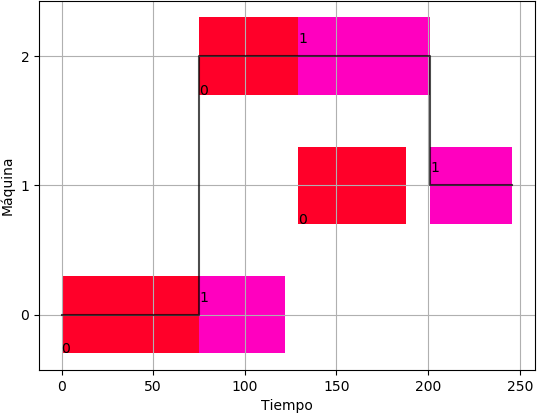
\includegraphics[scale=.7]{Imagenes/planejemplorc.png}
    \caption{Diagrama de Gantt de una planificación posible para la instancia mostrada en la tabla \ref{tab:inst2}. Se marcan los trabajos que pertenecen a la ruta crítica con una línea}
\label{fig:gantt2}
\end{figure}

Para recuperar la planificación previamente mostrada se asignan las llaves de la siguiente manera: \[k(O_{00})=k(O_{01})=k(O_{02})=1\]  \[k(O_{10})=k(O_{11})=k(O_{12})=0\]
\begin{itemize}
    \item Se inicializa $\Omega$ agregando las operaciones iniciales de cada trabajo, es decir:

\[\Omega = \{O_{10},O_{00}\}\]

     \item Se identifica a la operación que acabaría primero si se planifica ya, en este caso es $O_{10}$ que se debe procesar en la máquina $M_0$. 

     \item Se identifican las operaciones que podrían comenzar a procesarse antes del tiempo potencial de finalización de $O_{10}$. 
		 En este caso solo $O_{00}$ y  $O_{10}$ cumplen las condiciones.

Como $k(O_{00})>k(O_{10})$ se planifica $O_{00}$ se le asignan $0$ y $54$ como tiempos inicial y final.

     \item Se actualiza $\Omega$ eliminando a la operación planificada y agregando a su sucesora $O_{02}$.

\[\Omega\leftarrow \{O_{10},O_{02}\}\]
\end{itemize}
Este proceso continua de acuerdo al algoritmo \ref{alg:GT} hasta que todas las operaciones se encuentren planificadas.

\subsection{Construcción de soluciones activas a partir de no activas}

Realizar una búsqueda a partir de soluciones activas tiene la ventaja de moverse entre soluciones con una calidad media
superior.
%
Sin embargo, el proceso de generar las soluciones es costoso, por lo que tiene el inconveniente de analizar una menor
cantidad de soluciones candidatas, con respecto al caso en que no se aseguran que las soluciones son activas.
%
Por ello, es posible que utilizar un esquema en que se usen ambos tipos de representaciones de forma simultánea sea
ventajoso.
%
Con este fin, de diseñó una forma para movernos movernos entre soluciones de ambas representaciones, en concreto, para
generar una solución activa y su representación basada en llaves, a partir de una solución previa representada por una permutación que no tiene que ser activa. 

Para hallar la representación de alguna solución representada por una permutación se le asigna a cada operación una prioridad decreciente acuerdo a su posición de forma que se cumpla:
\[k(O_i)>k(O_{i+1})\]
\[\text{donde }O_i\text{ es la operación número $i$ en la representación basada en permutaciones}\]

Esta asignación nos asegura que se mantenga el orden de muchas operaciones pero convierte a la solución en activa. 
%
A continuación se muestra un ejemplo ilustrativo.

\subsubsection*{Ejemplo}
Consideremos la instancia del JSP mostrada en la siguiente tabla:
\begin{table}[H]
\centering
\begin{tabular}{@{}llll@{}}
Trabajo & \multicolumn{3}{l}{\begin{tabular}[c]{@{}l@{}}Secuencia de procesamiento \\ (máquina, tiempo)\end{tabular}} \\ \midrule
0 & 1, 37 & 0, 13 & 2, 35\\ \midrule
1 & 0, 8 & 1, 4 & 2, 9 \\\hline                         
2 & 1, 34 & 2, 72 & 0, 96 \\\hline                         
3 & 1, 63 & 0, 77 & 2, 24 \\\hline                         
\end{tabular}
\caption{Instancia 3 maquinas y 4 trabajos}
\label{tab:instactive}
\end{table}

La figura\ref{fig:nonactivepr} muestra un diagrama de Gantt para una posible planificación semi-activa.

\begin{figure}[H]
     \centering
     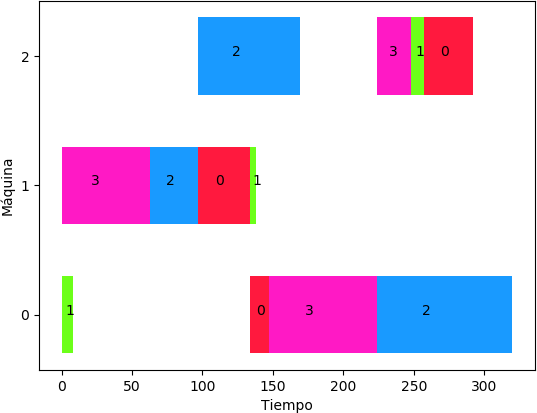
\includegraphics[scale=.7]{Imagenes/ganttnonactivepr.png}
     \caption{Planificación posible para la instancia en \ref{tab:instactive}. }
     \label{fig:nonactivepr}
\end{figure}
A partir de la planificación mostrada podemos asignar las prioridades del modo previamente dicho con lo que después de construir la planificación a partir de estas prioridades obtenemos la planificación que se muestra en la figura \ref{fig:activepr}.
\begin{figure}[H]
     \centering
     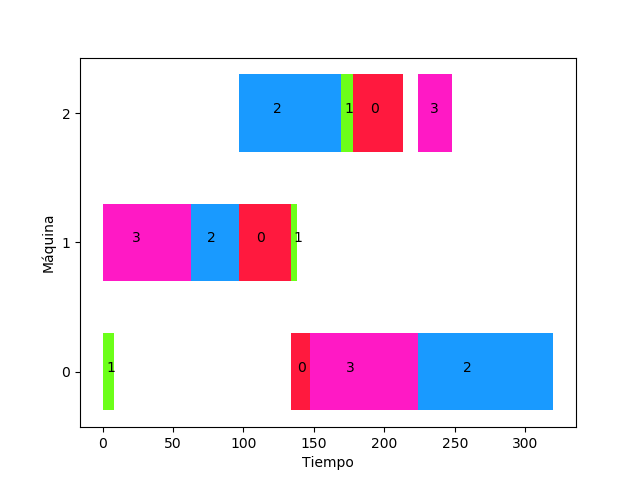
\includegraphics[scale=.7]{Imagenes/ganttactivepr.png}
     \caption{Planificación activa reconstruida a partir de la mostrada en la figura \ref{fig:nonactivepr}}
     \label{fig:activepr}
\end{figure}

Podemos notar como dos operaciones cambian de lugar de modo que se planifican antes sin aumentar el tiempo de inicio de otras aprovechando un hueco en el diagrama.

Una característica importante de esta representación es que el algoritmo usado para decodificar una solución activa a partir de las llaves numéricas considera en cada paso varias operaciones candidatas a planificar que cumplen con los criterios antes mencionados. Estas operaciones son la pieza en la que se basa la siguiente propuesta para una estructura de vecindad.
